\section{Der innovative Comp}
Der erste Eindruck zählt. Und Eindruck macht ein innovatives Unternehmen wie Digital Home nicht zuletzt durch entsprechende Innovationen.
Darauf wird hier gesetzt, weshalb bei der Website ein ungewöhnliches Konzept zum Einsatz kommt: horizontales Scrolling. Man findet es fast gar nicht auf anderen Websites, vor allem aus Rücksicht auf Desktopnutzer, die mit ihrer Maus meistens nur vertikal scrollen können. Das hat sich seit 2013 geändert, wo nun mehr als 50\% der Nutzer über Handhelds und Touchscreens auf das Internet zugreifen und außerdem das Touchpad durch Laptops weit verbreitet ist.
Die Startseite soll der erste Anlaufpunkt für Nutzer sein und soll daher eine kurze Produktübersicht enthalten. Trotz der Innovation wird hier auf das gewohnte Prinzip gesetzt, Content in aneinander gereihten Blöcken auf einer scrollbaren Seite zu präsentieren.

	\subsection{Comprehensive Dummy}

Eine erste Zeichnung des Comps hält die Grundidee fest (siehe Abbildung \ref{inno_Comp1}). Auf dieser Basis wird der Comp schrittweise zu einem fertigen Entwurf entwickelt.

\begin{figure} [hp]
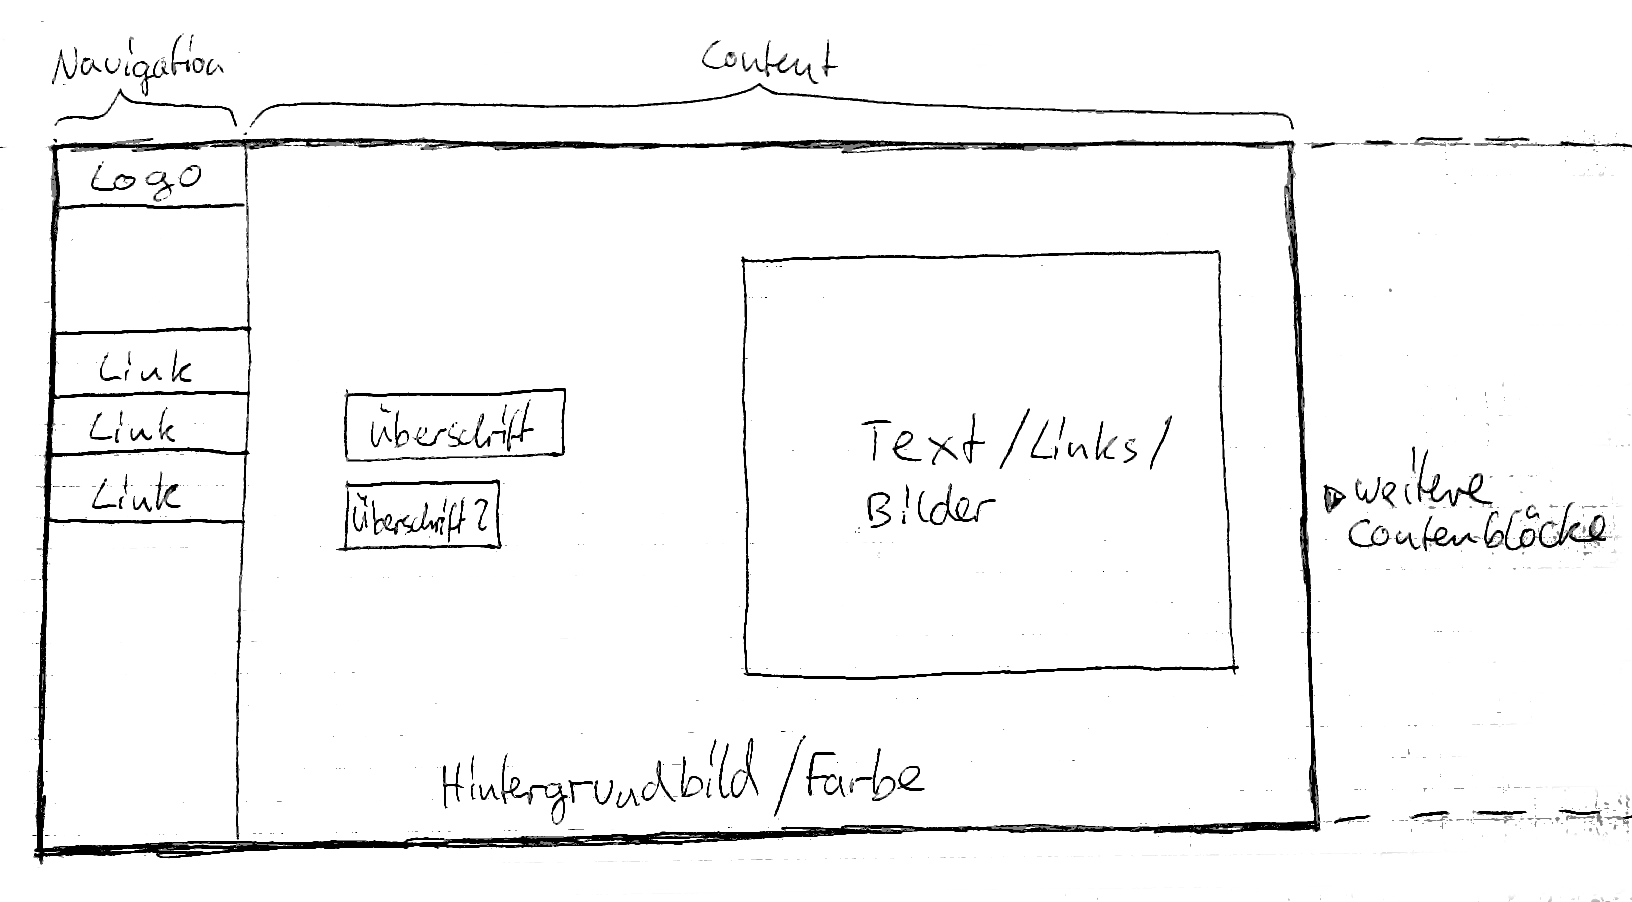
\includegraphics[width=\textwidth]{./img/inno_comp1.png}
\caption{Der erste Entwurf auf Papier}
\label{inno_Comp1}
\end{figure}
	\subsection{Entwicklungsphase HTML\&CSS}
\begin{figure} [tp]
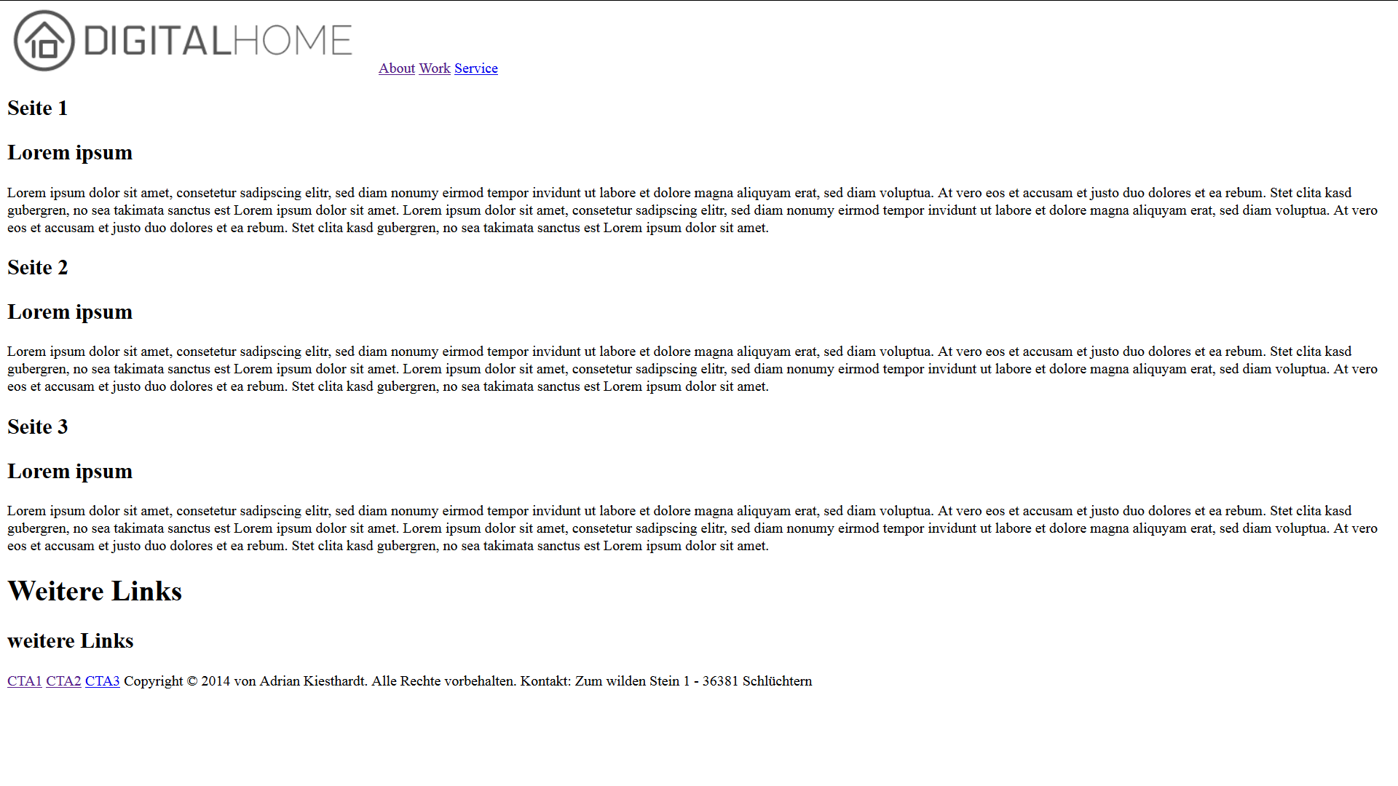
\includegraphics[width=\textwidth]{./img/inno_comp2.png}
\caption{Der erste Entwurf mit HTML}
\label{inno_Comp2}
\end{figure}
\begin{figure} [tp]
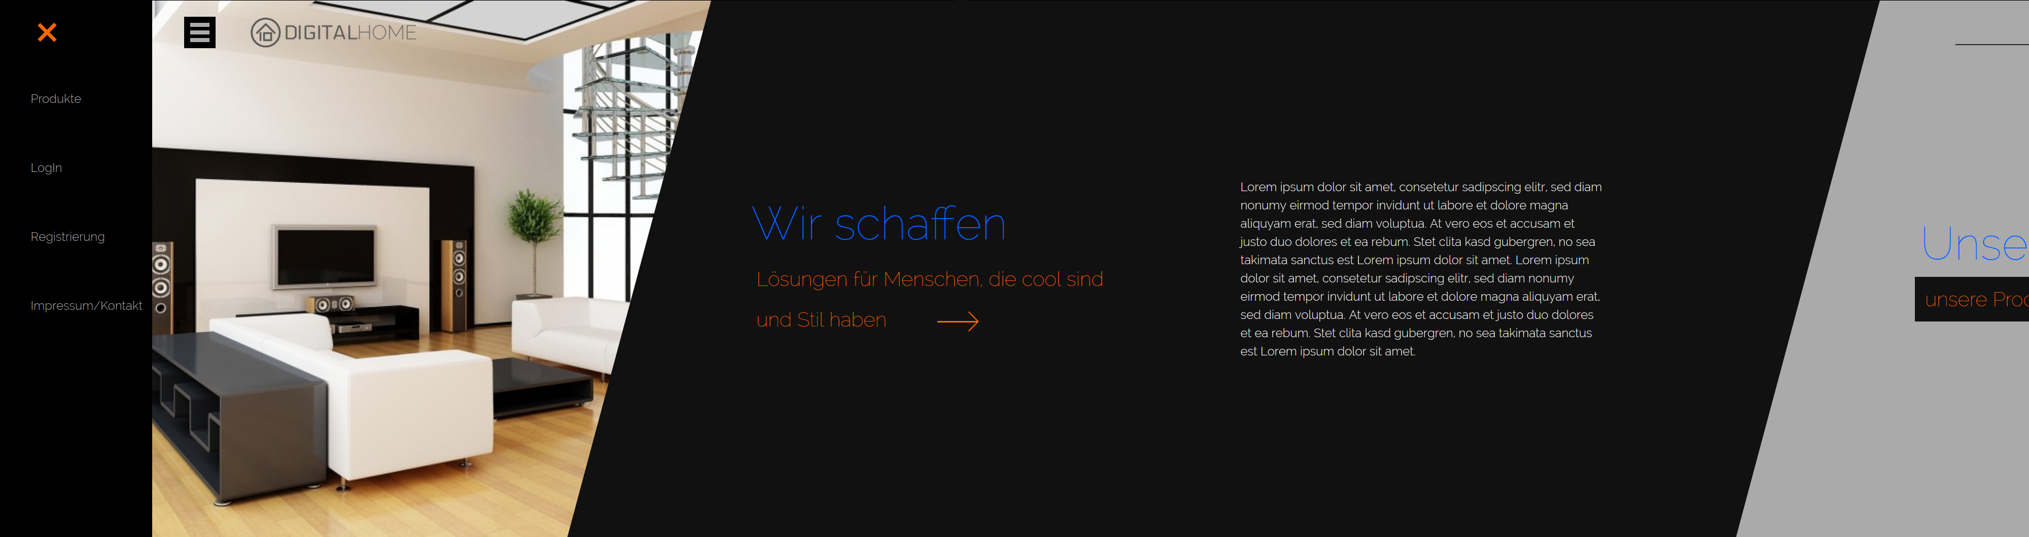
\includegraphics[width=\textwidth]{./img/inno_comp3.png}
\caption{Der erste Entwurf mit HTML\&CSS}
\label{inno_Comp3}
\end{figure}

Zur Umsetzung des horizontale Scrolling wäre es gut Tabellen zu verwenden, da diese die einzige sinnvolle Möglichkeit bieten, einen Container zu entwickeln, der sich abhängig vom Content nicht nach unten, sondern nach rechts erweitert (aufgrund der Eigenschaften von Tabellenzeilen). Da Tabellenlayouts mit <table> jedoch technisch hinter der Zeit, nicht responsive, unflexibel und semantisch falsch sind, braucht man eine Möglichkeit, das Tabellenlayout zu imitieren, ohne dabei Tabellen zu verwenden. Dazu werden in HTML die semantisch korrekten <section> Elemente verwendet (siehe Abbildung \ref{inno_Comp2}), die in CSS für das Tabellenlayout formatiert werden (siehe Abbildung \ref{inno_Comp3}). Die <section> Elemente werden als Tabellenzelle formatiert, die aufgrund der Organisation des <table> Elements in einer Zeile liegen. Der übergeordnete Container, der die Sections enthält, wird als Tabelle formatiert. Er breitet sich nach rechts aus und hat damit eine dynamische Breite. Die Sections haben jedoch eine relative Breite, die sich aufgrund des CSS bei Prozenteinheiten an dem übergeordneten Container orientieren würde, was nicht funktioniert. Die Container sollen ihre Größe an den Bildschirm anpassen, weshalb hier die Einheiten vw für „viewport width“ und vh für „viewport height“ eingesetzt werden.

	\subsection{Farbgebung\label{emo_col}}

Um der Innovation und Modernität gerecht zu werden, verwendet man Grautöne, hauptsächlich schwarz oder dunkle Grautöne. Da schwarz in enger Beziehung zum Tod steht, würde eine komplett schwarze Seite nicht einladend wirken. Wesentlicher eleganter wirkt Dunkelgrau. Schwarz lässt sich jedoch gut zur hierarchischen Abgrenzung spezieller Bereiche (z.B. Navigation) nutzen. Gleichzeitig muss ein Schwarzabgleich geschaffen werden, damit die Seite nicht zu hell wirkt und einen guten Kontrast bildet. Um diesen Kontrast nochmals zu unterstreichen, alterniert die Farbe des Hintergrunds. So entsteht ein Ausgleich zwischen dunklen und hellen Bereichen der Seite. Als Hintergrund wird also alternierend dunkelgrau/hellgrau, was seriös und einladend zugleich wirkt, und die Navigationsleiste wird schwarz. 

\begin{figure} [h]
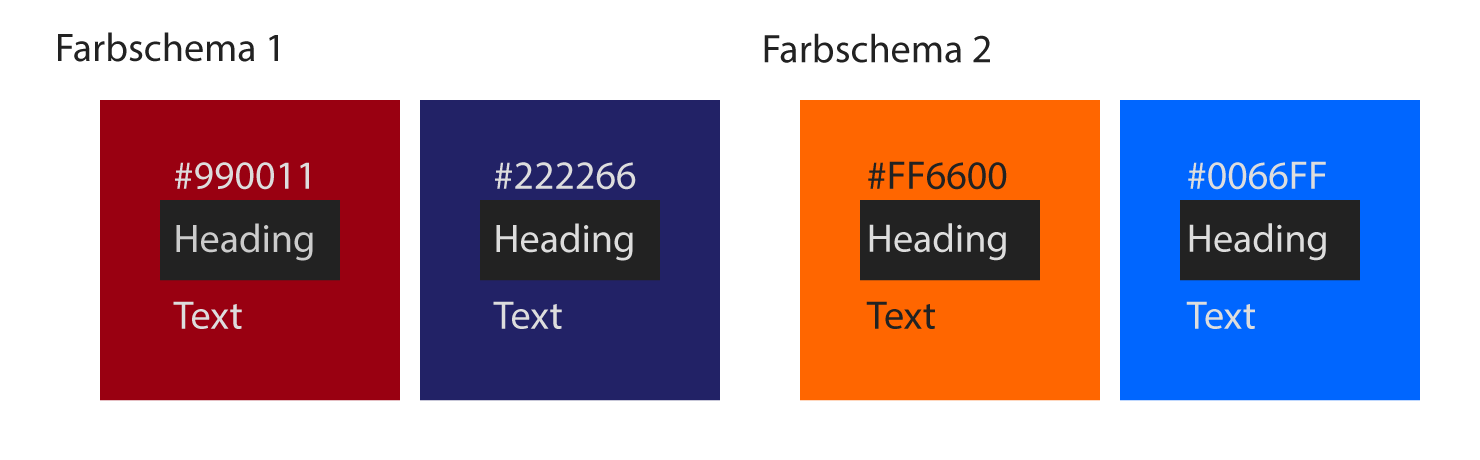
\includegraphics[width=\textwidth]{./img/inno_col1.png}
\caption{Diese Farbschemen kämen in Frage}
\label{inno_Farbschemen1}
\end{figure}


In grau wirkt die Seite ziemlich trist, deswegen kommen Akzentfarben zum Einsatz. Mehr als zwei Farbtöne sind zu bunt, ein einzelner Farbton belastet die Wirkung einseitig. Deshalb werden zwei Farben gewählt. Pastellfarben wirken seriös und edel, so kommt das erste Farbschema aus einem emotionalen rot und einem ruhigen, dunklen blau zu Stande. Das zweite Farbschema besteht aus stechenden Farben (siehe Abbildung \ref{inno_Farbschemen1}). Das wirkt künstlerisch, dynamisch, modern und kreativ. Orange ist zudem die Farbe der Kreativität. Als Ausgleich wird hier Himmelblau eingesetzt, das durch die direkte Assoziation mit dem Himmel Freiraum und Großzügigkeit vermittelt, aber auch kühl, technisch wirkt. In den zwei Farbschemen stehen sich ein warmer Farbton und ein kalter Farbton in ungefähr gleicher Helligkeit und Sättigung gegenüber, wodurch eine kontrastreiche und dennoch eine ausgeglichene, ruhige, unaufdringliche Atmosphäre entsteht.

\begin{figure} [h]
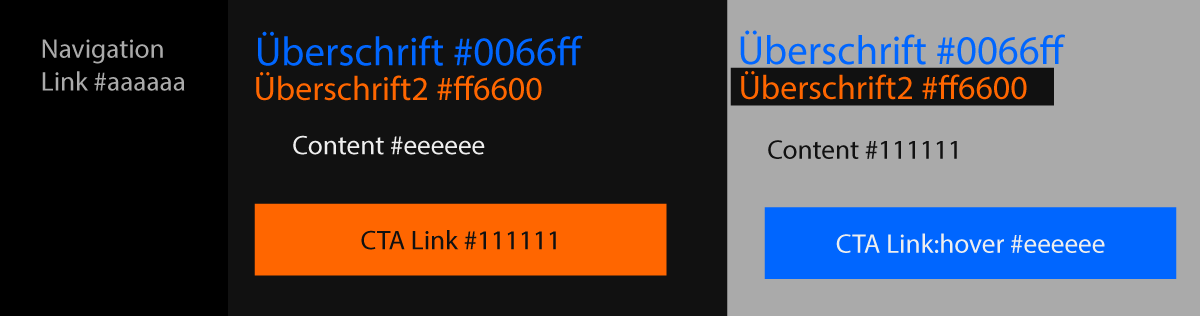
\includegraphics[width=\textwidth]{./img/inno_col2.png}
\caption{Das zweite Farbschema}
\label{inno_Farbschemen2}
\end{figure}

Der Grund, sich für das zweite Farbschema zu entscheiden, liegt darin, dass sowohl das erste als auch das zweite den Farbverlauf des Himmels gegen Abend wiederspiegeln. Das bindet den Menschen im Allgemeinen emotional, viele empfinden den Sonnenuntergang als romantisch. Das erste Farbschema drückt dieses Gefühl in einer sehr ruhigen Weise aus, stellt jedoch auf Grund der fehlenden Sättigung eher den Teil des Abends da, wenn die Sonne bereits untergegangen ist. Am stärksten ist das Gefühl zu jenem Zeitpunkt, an dem sich der Himmel blau und orange färbt, wie im zweiten Farbschema. Dazu kommt, dass blau und orange auf dunklem Hintergrund besser zu lesen sind als dunkel rot und dunkel blau und das Menschen mit Rot-Grün-Schwäche orange im Gegensatz zu dunkel rot erkennen können. Daher wird hier das 2.Farbschema als Hauptfarbschema gewählt (siehe Abbildung \ref{inno_Farbschemen2}).
Ein bleibendes Problem ist der weiße Text auf schwarzem Hintergrund, der die Augen mehr belastet als schwarzer Text auf weißem Hintergrund. Jedoch bietet sich dunkler Hintergrund bei bildlastigen Seiten an wegen des Fehlens von störenden weißen Rändern um Bildern. Außerdem relativiert sich das Problem durch die geringe Textmenge und die alternierende Hintergrundfarbe.


	\subsection{Typographische Gestaltung} 
	\label{typo_inno}

Die Qualität des Designs wird vor allem durch das Zusammenspiel der einzelnen Faktoren bestimmt. Zu dem Layout und den Farben muss auch die Typografie passen. Dazu wurden Typefaces gesucht, die zum modernen und kreativen Auftreten von Digital Home und damit der Website passen. Da dem Projekt zurzeit keine kommerziellen Fonts zur Verfügung stehen, musste die Suche auf frei zugängliche Schriftarten beschränkt werden. Unter Rücksicht auf die Ladezeiten der Website und das Cachen der Fonts wurde hier Google Fonts als CDN für die gesuchten Typefaces gewählt.
Da die gesuchte Schriftart innovativ und technisch wirken soll, kann die Suche auf Sans-serifs beschränkt werden. Außerdem sollen durch dünne Linien Minimalismus und Reinheit betont werden. Unter jenen Sans-serif Schriftarten findet sich Raleway, welches sich selbst als Humanist-Sans bezeichnet. Dieser Teil der Font-Familie (Raleway Light bzw. Thin) hat jedoch auch stilistische Eigenschaften einer Geometric-Sans Font, welche in Architektur und Wissenschaft \footcite[vgl.][]{codeschool:typo} sehr beliebt sind. Zwischen diesen beiden Typen liegen die Transitional-Sans. Diese sind gut mit den Themen Technologie und Wirtschaft zu verbinden. Architektur und Technologie sind eben jene zwei Kernbereiche der Digital-Home-Idee, weshalb sich diese Font letztlich so gut eignet.
        \begin{figure} [htp]
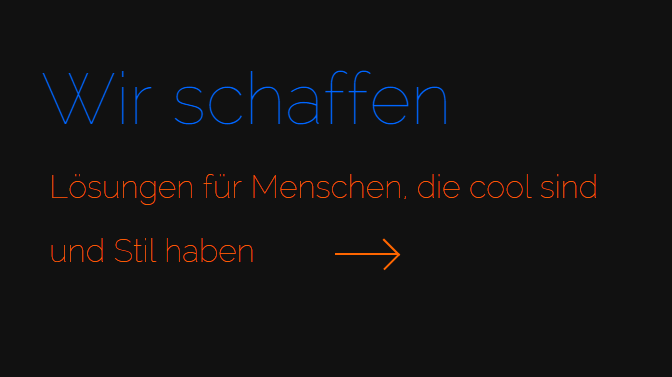
\includegraphics[width=\textwidth]{./img/inno_typo1.png}
\caption{Unterüberschrift mit Fontdicke 100}
\label{inno_Typo1}
\end{figure}

        \begin{figure} [htp]
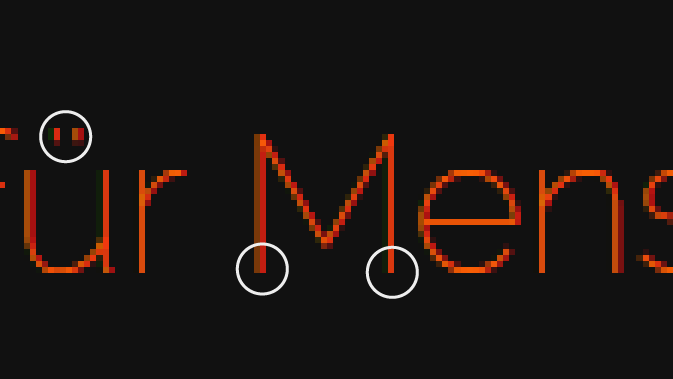
\includegraphics[width=\textwidth]{./img/inno_typo1_2.png}
\caption{Bei der Dicke 100 treten unangenehme Effekte auf, weil sich Linien teilweise zwischen Pixel bewegen. Durch die Kantenglättung entstehen dann ungleichmäßig dicke Linien bzw. Punkte (Im Bild weiß makiert)}
\label{inno_Typo12}
\end{figure}

\begin{figure} [htp]
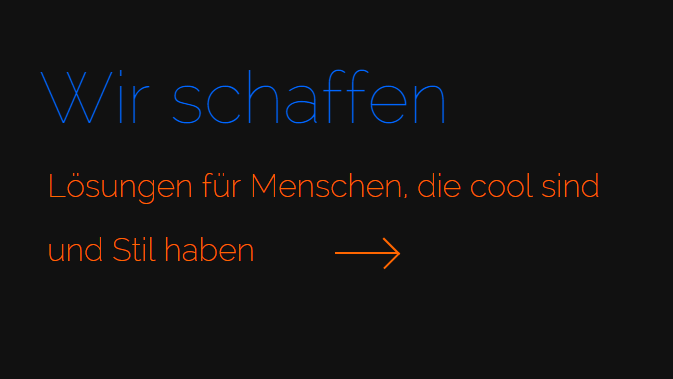
\includegraphics[width=\textwidth]{./img/inno_typo2.png}
\caption{Unterüberschrift mit Fontdicke 200}
\label{inno_Typo2}
\end{figure}
Das Ziel, eine möglichst dünne Font zu verwenden, muss aus Gründen der Lesbarkeit eingeschränkt werden. Während die Fontdicke 100 bei Überschriften gut funktioniert (siehe Abbildung \ref{inno_Typo1}), treten bei den Unterüberschriften unangenehme visuelle Effekte auf (siehe Abbildung \ref{inno_Typo12}), weshalb hier die Dicke auf 200 gesetzt wurde (siehe Abbildung \ref{inno_Typo2}). Textblöcke mit noch kleinerer Schrift bekommen die Dicke 300.


	\subsection{Strukturanalyse der Seite}

Da das Augenmerk beim Webdesign trotz der ungewöhnlichen Idee trotzdem auf Usability liegt, sollte das Wichtigste oben links stehen, nämlich wo der Nutzer sich befindet und wie er weiterkommt. Deshalb wird der Menubutton und das Logo in die linke obere Ecke verschoben. Beim Klick auf den Menubutton wird das Menu, welches OffCanvas und auch links liegt, von links eingefahren. Dadurch wird der Bezug zwischen dem Button und dem Menu selber hergestellt und Konsistenz wird gewahrt \footcite[vgl.][]{MaterialD:menu}.
 \begin{figure} [htp]
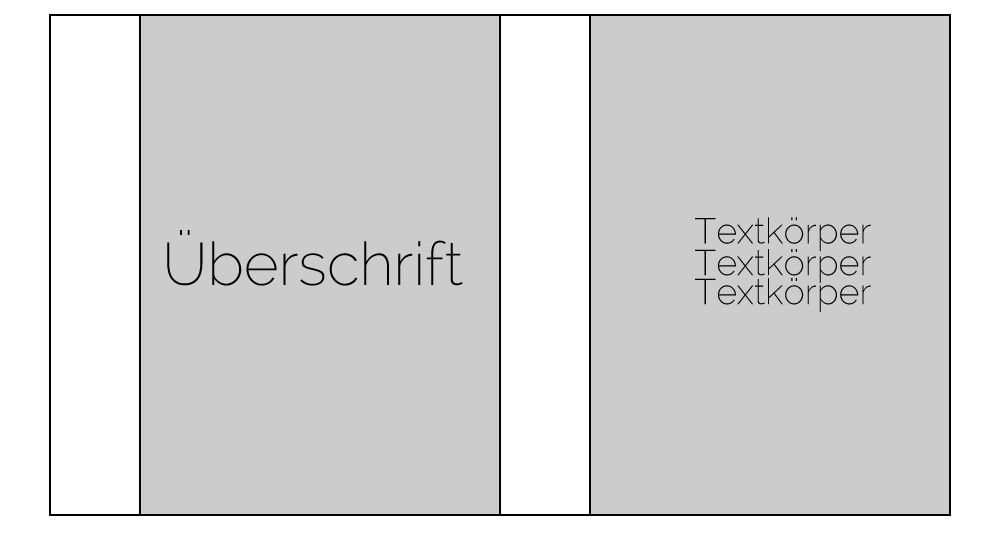
\includegraphics[width=\textwidth]{./img/inno_struct1.png}
\caption{zweispaltiges Layout}
\label{inno_Struct1}
\end{figure}
Das Wichtigste an der Website ist der Content, in diesem Falle sind das Texte und Bilder, die sehr sparsam eingesetzt werden. Deshalb kommt hier viel Whitespace zum Einsatz. Um den Content zu strukturieren, wird der einzelne Contentblock in der Mitte geteilt (siehe Abbildung \ref{inno_Struct1}). In dieser halben „Seite“ kann ein Bild, eine Überschrift oder Text stehen. Der Content wird vertikal zentriert, damit sich der Whitespace gleichmäßig verteilt.

Stellt man die Sections als rechteckige Container dar, so wirkt die Kante zwischen den Sections beim Scrollen wie eine abrupt auftauchende Wand, die den Beginn eines neuen Abschnittes ankündigt. Deshalb kommen schräge Linien zum Einsatz, um das Design ein aufzubrechen [Inspiration: Dekonstruktivismus in der Architektur] und kommende Sections sanft einzuleiten. Hier soll damit vor allem erreicht werden, dem Design trotz seines simplen Aufbaus etwas Komplexes zu geben, damit es nicht langweilig wirkt und der Nutzer durch den entstehenden Überraschungseffekt länger an der Stange gehalten wird. Nach Tests im Bezug auf die Innen-und Außenabstände der Sections wurde sich hier auf eine $15\,^{\circ}{\rm}$ Neigung im Uhrzeigersinn geeinigt. Durch die dennoch gradlinigen Kanten bekommt die Seite einen Look, der gut mit der klinischen Atmosphäre der Farben harmoniert. 


Auf jeder Seite der Website soll als erstes ein Titelbild sein, um dem Nutzer schnell das Thema der Seite zu erklären. Redundant befindet sich auf der rechten Seite eine Überschrift, damit der Nutzer sichergehen kann, dass er sich auf der richtigen Seite befindet. Das sind die einzigen Bereiche, die above the fold liegen. Zusätzlich ist die Überschrift von reichlich Whitespace umgeben, damit sich der Nutzer nicht ablenken lässt. Beim Weiterscrollen schließt sich direkt der restliche Content an.
Aufgrund der Preise der Produkte sowie der Seriosität, die über die Seite vermittelt werden soll, wird auf Werbung verzichtet. Außerdem werden auf der Startseite keine Preisschilder angezeigt, um nicht aufdringlich zu wirken.
\label{inno_probs}
Probleme dieses Designs zeigen sich in den schrägen Elementen im Produkt Abschnitt. Die schrägen Links haben auf Grund von Kantenglättungsschwierigkeiten einen weißen Rand (Rendering), der hier durch einen 1px dicken schwarzen Rand (CSS) unterbunden wurde. Außerdem ist das Layout ziemlich unflexibel, da die Breite der Seite von der Anzahl der Elemente abhängen sollte, sich jedoch nicht dynamisch anpassen kann und daher separat geändert werden muss. Das bedeutet unnötigen Wartungsaufwand, der sehr schnell zu Schwierigkeiten (z.B. Bugs, Inkonsistenzen) führen kann.
Punkten kann dieser Entwurf jedoch mit seiner aufgeräumten Struktur, dem sehr innovativen Menübutton und dem ungewohnten Scrollverhalten.
